\section{Cosa si intende per serie di Fourier?}
Un segnale che ha una durata finita può essere gestito immaginando semplicemente che esso ripeta infinite volte l’intero schema (intervallo T e 2T è identico all’intervallo 0 a T).

È possibile quindi rappresentare i segnali tramite funzioni, le quali permettono un’analisi e una modellazione più efficace.
La Serie di Fourier non è altro che la scomposizione di un segnale in componenti sinusoidali (possibilmente infiniti).

%\begin{figure}[H]
%\centering
%\includegraphics[scale=1]{../img/.png}
%\caption{Didascalia dellimmagine}
%\end{figure}

$f=1/T$ rappresenta la frequenza fondamentale, $a_n$  $b_n$  sono rispettivamente le ampiezze seno e coseno dell’n-esima armonica e \textit{c} rappresenta una costante.

Su questo teorema si basano le reti e il passaggio dei dati tramite i mezzi di trasmissione; purtroppo 	nella pratica i mezzi di trasmissione attenuano in modo non uniforme i componenti della serie di Fourier, generando così una distorsione. Per ovviare a questa distorsione, le ampiezze fino ad una certa frequenza vengono trasmesse senza modifiche, da quella frequenza in poi vengono attenuate.

L’intervallo di frequenze trasmesse senza una forte attenuazione è chiamato Banda Passante.
Generalmente nella realtà viene indicata la banda passante compresa tra 0 e la frequenza dove la potenza è attenuata del 50\%.
\section{Bitrate e Baudrate}

Il Bitrate è la quantità di informazioni digitali che è trasferita o registrata nell’unita di tempo.
Stiamo parlando quindi di velocità di trasmissione, espressa in bit/s. La velocità di trasmissione è anche detta Banda. La velocità di trasmissione dipende dal tipo di mezzo trasmissivo utilizzato e dalle sue condizioni fisiche al momento dell’uso.

Il Baudrate invece rappresenta il numero di simboli che viene trasmesso in un secondo. Non va confusa con il sopracitato bitrate in quanto misurano unità differenti, infatti ad un simbolo corrisponde un numero di bit differente in base alle tecniche di modulazione utilizzate.

\section{Descrivere i vari tipi di cavo e confrontarli}
I principali tipi di cavo utilizzato nelle telecomunicazioni sono: il doppino, il cavo coassiale e la fibra ottica. \\
\textbf{Il doppino}:\\
-Cos’è: è un cavo composto da due conduttori di rame isolati, spessi circa 1mm e avvolti uno intorno all’altro in una forma elicoidale. L’intreccio è utile per annullare i campi elettromagnetici generati dai due conduttori, i quali si annullano a vicenda. Esistono diverse varietà di doppini, i più importanti per le telecomunicazioni sono gli UTP3 e UTP5, (UTP= Unshielded Twisted Pair, doppini non schermati), Le differenze tra i doppini di categoria 3 e categoria 5 sta nel numero di spire per centimetro, minor numero di spire per cm negli UTP3 e maggiore negli UTP5, un maggior numero di spire permette di migliorare la qualità del segnale trasmesso su lunghe distanze, a scapito però della quantità di materiale necessario. Esistono anche categorie superiori, i quali gestiscono segnali con banda più ampia.  \\

\begin{figure}[H]
\centering
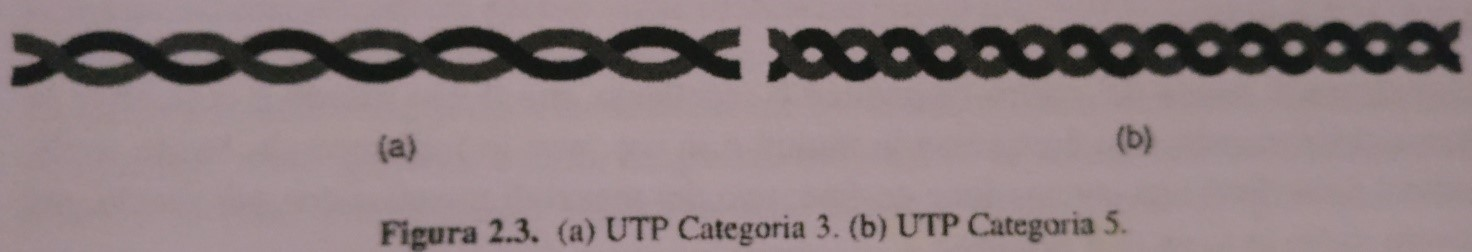
\includegraphics[scale=0.7]{res/img/3_Doppino.jpg}
%\caption{Didascalia dell'immagine}
\end{figure}
-Applicazione: Il sistema di applicazione più diffuso per il doppino è il sistema telefonico. I doppini si 	possono utilizzare per trasmettere segnali analogici e digitali, l’ampiezza di banda dipende dal diametro del cavo e dalla distanza percorsa. Sono molto utilizzati grazie al basso costo e al discreto livello di prestazioni. \\
\textbf{Il cavo coassiale}: \\
-Cos’è: è un cavo composto da un nucleo conduttore coperto da un rivestimento isolante, a sua volta circondato da un conduttore cilindrico, solitamente realizzato con una calza di conduttori sottili, che infine è avvolto da una guaina protettiva di plastica. La costruzione e la schermatura del cavo coassiale forniscono ampiezza di banda ed eccellente immunità al rumore. Ne esistono di due tipi, a 50$\Omega$ per le trasmissioni digitali e a 75$\Omega$ per quelle analogiche, non c’è una motivazione tecnica per questa distinzione.\\
-Applicazione: Il cavo coassiale è molto utilizzato per le reti metropolitane e le televisioni via cavo, la banda disponibile dipende dalla qualità, dalla lunghezza del cavo e dal rapporto segnale-rumore del segnale dati. Per molti ambiti il cavo coassiale è stato sostituito dalla fibra ottica per i tratti più lunghi.

\begin{figure}[H]
\centering
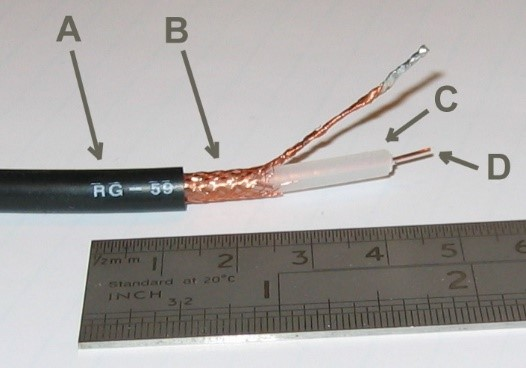
\includegraphics[scale=1]{res/img/3_cavoCoassiale.jpg}
%\caption{Didascalia dell'immagine}
\end{figure}
D: nucleo, C: rivestimento isolante, B: conduttore cilindrico, A: guaina protettiva. \\
\textbf{Fibra ottica:}\\
-Cos’è: Un sistema di trasmissione ottico è formato da: sorgente luminosa, mezzo di trasmissione e rilevatore. I cavi in fibra ottica è il mezzo di trasmissione di questo sistema, che si basa su segnali luminosi invece che elettrici.
La fibra ottica è formata da un nucleo (core) di vetro, attraverso il quale si propaga la luce, ha uno spessore di 50 micron per le fibre multimodali mentre dagli 8 ai 10 micron per quelle monomodali.

Il nucleo è avvolto da un rivestimento di vetro (cladding) che ha un indice di rifrazione più basso; ciò costringe la luce a rimanere nel nucleo. L’ultimo strato è formato da plastica e serve a proteggere il rivestimento. Generalmente le fibre sono raggruppate in fasci, protetti da un’ulteriore guaina più esterna.  

\begin{figure}[H]
\centering
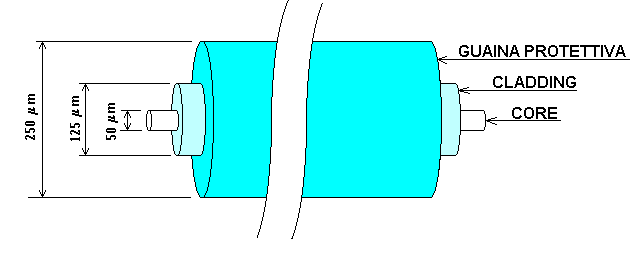
\includegraphics[scale=0.7]{res/img/3_FibraOttica.png}
%\caption{Didascalia dellimmagine}
\end{figure}

Esistono due tipi di fibra, la monomodale e la multimodale. La monomodale è più costosa e utilizzata soprattutto per le lunghe distanze, in cui la luce può propagarsi solo in linea retta senza rimbalzare.
Nella multimodale invece può contenere più raggi che rimbalzano ad angoli diversi, in questo caso si dice che ogni raggio ha una modalità diversa, da qui il nome multimodale.

Le fibre si possono collegare in diversi modi:
\begin{itemize}
\item Tramite connettori in apposite prese, perdono il 10-20\% di luce ma semplificano la riconfigurazione dei sistemi. 
\item Attaccate meccanicamente, tramite una manichetta speciale viene pinzato, viene poi allineato in modo da massimizzare il segnale, perdita del 10\% 
\item Fusione delle due parti, genera una piccola attenuazione.
\end{itemize}
-Applicazione: La fibra è molto utilizzata nelle LAN e nei sistemi di trasmissioni a lunga distanza e apporta diversi vantaggi rispetto al cavo in rame:
\begin{itemize}
\item	Maggiore ampiezza di banda.
\item	I ripetitori possono essere installati ogni 50km rispetto all’ogni 5km dei cavi in rame, con un evidente risparmio.
\item	Non è influenzata da sorgenti elettriche, dai campi elettromagnetici e dalle interruzioni della linea elettrica, la fibra è adatta anche agli ambienti più inospitali.
\item	La fibra è sottile e leggera, occupando meno spazio permette alle aziende telefoniche di svuotare i condotti ormai saturi di cavi.
\item	Le fibre non perdono la luce ed è difficile intercettare i dati, questo le rendono molto più sicure rispetto ai cavi in rame.
\end{itemize}
Presenta tuttavia dei svantaggi, che nonostante tutto non limitano troppo questa tecnologia, che rappresenta il futuro per le telecomunicazioni. Tra gli svantaggi troviamo:
\begin{itemize}
\item	Tecnologia meno nota, richiede conoscenze che non tutti gli ingegneri possiedono.
\item	Si può danneggiare se la si piega troppo.
\item	La trasmissione è unidirezionale, di conseguenza, per avere una comunicazione bidirezionale è richiesta una doppia fibra o due bande di frequenza in una sola.
\item	Le interfacce per la fibra ottica costano di più di quelle elettriche.
\end{itemize}


\section{Caratteristiche e confronto tra i vari tipi di satellite: GEO, MEO e LEO}

Un satellite di comunicazioni può essere immaginato come un grande ripetitore di microonde posto nel cielo. Questo dispositivo contiene diversi transponder, ossia ricetrasmettitori satellitari, i quali ascoltano una parte dello spettro, amplificano il segnale e lo ritrasmettono su altre frequenze per evitare interferenze.
La collocazione dei satelliti è importante, e determinata da alcuni fattori:
\begin{itemize}
\item	Il periodo orbitale: più alto è il satellite, più lungo è il periodo.
\item	Le fasce di Van Allen distruggerebbero velocemente un satellite che le attraversasse.
\end{itemize}
Esistono quindi 3 zone in cui i satelliti possono essere collocati LEO: sotto la fascia di Van Allen inferiore, MEO: tra la fascia VA inferiore e quella superiore, e i GEO: molto al di sopra della fascia VA superiore.

\begin{figure}[H]
\centering
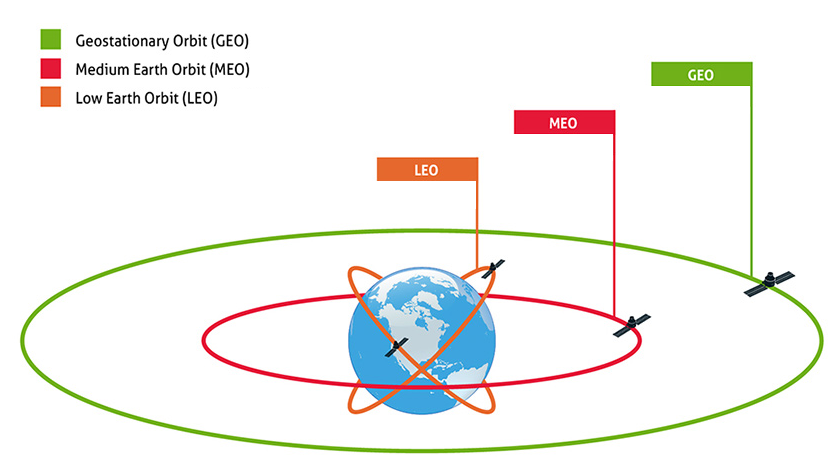
\includegraphics[scale=0.55]{res/img/4_satelliti.png}
%\caption{Didascalia dellimmagine}
\end{figure}
 
\paragraph{GEO}
GEO (Geostationary Earth Orbit), sono collocati nella fascia più alta, disposti con un intervallo di $2^{\circ}$ nel piano equatoriale, così da evitare interferenze, di conseguenza c’è posto per “solo” 180 satelliti di questo tipo, la loro dimensione è importante e la gestione dell’allocazione degli slot orbitali è motivo di disputa tra paesi, stazioni televisive e militari.
\paragraph{MEO}
Tra le due fasce di Van Allen troviamo i satelliti MEO (Medium Earth Orbit), questi satelliti si spostano lentamente lungo la longitudine, impiegando 6 ore per compiere un giro attorno al pianeta, attualmente non sono utilizzati per le telecomunicazioni. Rispetto al GEO, il MEO permette un ritardo di propagazione inferiore, tuttavia si perde la comodità del “punto fisso” garantito dal GEO, questo perché il MEO si sposta più velocemente.
\paragraph{LEO}
I LEO (Low Earth Orbit) sono I più bassi tra i tre tipi, si spostano molto velocemente, di conseguenza un sistema completo richiede l’utilizzo di molti satelliti di questo tipo. D’altra parte, le stazioni terrestri non hanno bisogno di molta energia per la comunicazione e i ritardi sono di pochi millisecondi.
Questo tipo di satellite tratta prevalentemente trasmissione voce e servizi internet/GPS. \\

Una menzione particolare va fatta alla differenza tra satelliti e fibra, quale preferire? 
Non esiste una risposta ben definita, la fibra grazie alla sua comodità sembrava avesse preso dominio nel mercato, tuttavia i satelliti avevano applicazione in campo in cui la fibra non poteva arrivare:
\begin{itemize}
\item	La fibra non è attualmente disponibile a una gran parte dell’utenza, mentre per i satelliti, l’utente basta che innalzi un’antenna sul tetto di casa per ottenere una maggiore ampiezza di banda.
\item	Comunicazione mobile, la fibra ottica non è di nessuna utilità per questa categoria, mentre i collegamenti satellitari potenzialmente ce l’hanno.
\item	Comunicazione broadcast, un messaggio inviato da un satellite può essere ricevuto contemporaneamente da migliaia di stazioni terrestri.
\item	Comunicazione in luoghi con terreni inospitali o scarsamente dotati di infrastrutture.
Il sistema di comunicazione principale del futuro sarà quello terrestre basato su fibre ottiche, combinato con la rete radio cellulare, tuttavia per alcune applicazioni specifiche i satelliti sono migliori.
\end{itemize}

\section{Cos’è la modulazione in frequenza?}
Durante l’invio di informazioni, il segnale può subire attenuazione, distorsione o venir disturbata dal rumore; questo porta ad evitare l’uso di un largo intervallo di frequenze, ma sfortunatamente le onde quadre utilizzate nei segnali digitali utilizzano un ampio spettro di frequenza, e perciò sono soggette ad una forte attenuazione e alla distorsione.

Questi effetti portano adatta la trasmissione in banda base (DC) solo a velocità basse e distanze brevi.
Per aggirare questi problemi viene usata la trasmissione AC, un tono continuo(portante d’onda sinusoidale) nell’intervallo compreso tra 1000 e 2000Hz, il quale permette la modulazione della sua ampiezza(AM), frequenza(FM) o fase.

\begin{figure}[H]
\centering
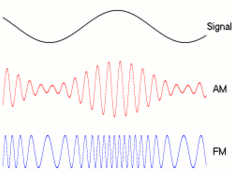
\includegraphics[scale=1]{res/img/5_modulazione.png}
%\caption{Didascalia dellimmagine}
\end{figure}
 
La modulazione in frequenza non è altro che una tecnica di trasmissione utilizzata per trasmettere informazioni usando la variazione di frequenza dell’onda portante. Rispetto alla modulazione in ampiezza ha il vantaggio di essere molto meno sensibile ai disturbi e permette una trasmissione di miglior qualità. Ha inoltre un’efficienza energetica molto maggiore dato che la potenza del segnale modulato FM è esclusivamente quello della portante.

Il difetto principale è la necessità di circuiti più complessi, sia per la generazione del segnale sia per la ricezione. L’attuale tecnologia ha permesso di superare queste problematiche, rendendo la modulazione in frequenza molto più usata rispetto a quella in ampiezza, soprattutto in ambito di broadcasting commerciale.

\section{Cos’è la modulazione delta (delta modulation)?}
La delta modulation è un metodo di digitalizzazione e compressione di un segnale analogico.
Si basa sul fatto che il segnale cambia in modo relativamente lento rispetto alla frequenza di campionamento, ciò rende gran parte dell’informazione ridondante.

Questo metodo prevede che ogni valore campionato differisca dal precedente di +1 o -1, sotto queste condizioni è possibile trasmettere un singolo bit che dice se il nuovo campione è maggiore o minore del precedente.

Un problema si ha se il segnale cambia troppo rapidamente, in quel caso si perdono informazioni.

\begin{figure}[H]
\centering
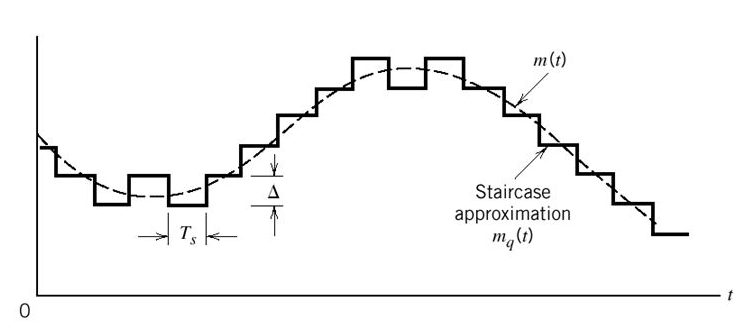
\includegraphics[scale=0.6]{res/img/6_modulazioneDelta.png}
%\caption{Didascalia dellimmagine}
\end{figure}
 
\section{Descrivere in dettaglio il GSM (Global System for Mobile connection)}
Esistono tre generazioni distinte di telefoni cellulari ognuna caratterizzata da una diversa tecnologia:
\begin{itemize}
\item	Voce analogica
\item	Voce digitale
\item	Voce e dati digitali (Internet, posta elettronica ecc.)
\end{itemize}
Il GSM tratta dei telefoni della seconda generazione: voce digitale.

La sua struttura è formata da 4 tipi di celle: macro, micro, pico e umbrella. 
Le prime sono le più grandi, sono sopraelevate rispetto gli edifici e hanno un raggio massimo si 35 km. Le micro sono più piccole, coprono un'altezza pari agli edifici. Le pico sono molto piccole, usate in aree molto dense, tipicamente indoor. Umbrella è una piccola estensione, usata per coprire i buchi tra le varie celle sopracitate.

Sfrutta il multiplexing a divisione di frequenza, con ogni apparecchio che trasmette su una frequenza e riceve su una frequenza più alta. Una singola coppia di frequenza è divisa in slot temporali e condivisa tra più utenti attraverso un meccanismo di multiplexing a divisione di tempo.

Questi fattori lo rendono molto simile al D-AMPS, tecnologia molto utilizzata in America, che condivide la stessa generazione di telefoni. Tuttavia, GSM sono molto più ampi di quelli AMPS e contengo un numero poco più alto di utenti, perciò la velocità dati per utente di GSM è superiore a quella di D-AMPS.

Un sistema GSM ha 124 coppie di canali simplex e supporta otto connessioni separate mediante multiplexing a divisione di tempo.
A ogni stazione attiva è assegnato uno slot temporale su una coppia di canali.

Trasmissione e ricezione non avvengono nello stesso intervallo temporale perché GSM non è in grado di trasmettere e ricevere contemporaneamente.

Il GSM introduce anche l’utilizzo della SIM card, in cui vengono memorizzati i dati descrittivi dell’abbonato e ha la funzione principale di fornire autenticazione ed autorizzazione all’utilizzo della rete.

\section{Si descriva la tecnica CDMA (Code Division Multiple Access), possibilmente con esempio}
Esistono tre generazioni distinte di telefoni cellulari ognuna caratterizzata da una diversa tecnologia:
\begin{itemize}
\item	Voce analogica
\item	Voce digitale
\item	Voce e dati digitali (Internet, posta elettronica ecc.)
\end{itemize}
Il CDMA tratta dei telefoni della seconda generazione: voce digitale.

D-AMPS e GSM sono sistemi che utilizzano FDM e TDM per dividere lo spettro in canali e i canali in slot temporali. CDMA invece di dividere l’intero intervallo di frequenze assegnate in poche centinaia di canali a banda stretta, permette ad ogni stazione di trasmettere per tutto il tempo attraverso l’intero spettro di frequenza. Trasmissioni multiple simultanee sono separate usando la teoria della codifica. La capacita del CDMA è di riuscire a estrarre il segnale desiderato scartando tutto il resto.

In CDMA, ogni tempo bit è suddiviso in m intervalli chiamati chip. In genere ci sono 64 o 128 chip per ogni bit. Ad ogni stazione è assegnato un codice di m-bit univoco chiamato sequenza di chip.
Per trasmettere un bit 1, una stazione invia la sua sequenza di chip; per trasmettere un bit 0 la stazione invia il complemento a uno della propria sequenza di chip.
Ogni stazione adotta una sequenza di chip univoca.

CDMA rispetto a GSM e D-AMPS opera in una banda di 1,25MHz, permettendo agli utenti di avere un’ampiezza di banda considerevole.
Una sequenza di chip e il suo contrario sono a due a due ortogonali (il prodotto interno normalizzato è 0). Per generare queste sequenze di frammento ortogonali si utilizza un metodo noto come codici Walsh. 
Se la sequenza di chip ricevuta è S e il ricevitore sta cercando di ascoltare una stazione la cui sequenza di chip è C, il prodotto interno normalizzato da calcolare è S*C; facendo i calcoli si possono eliminare i termini superflui grazie all’ortogonalità dei valori, estraendo correttamente il valore trasmesso da C. 
Ad esempio, A e C trasmettono 1, B trasmette 0. Il ricevitore vede la somma S=A+!B+C e calcola:\\
$S*C=(A+!B+C)*C=A*C+B*C+C*C=0+0+1=1$ \\
I primi due termini spariscono perché le sequenze di chip sono state scelte per essere ortogonali.

\section{Il GPRS: Cos’è? Pregi e difetti}

Esistono tre generazioni distinte di telefoni cellulari ognuna caratterizzata da una diversa tecnologia:
\begin{itemize}
\item	Voce analogica
\item	Voce digitale
\item	Voce e dati digitali (Internet, posta elettronica ecc.)
\end{itemize}
GPRS è un’evoluzione tra la seconda e la terza generazione di telefoni cellulari. È una rete a pacchetti costruita sopra D-AMPS e GSM. Questa permette alle stazioni mobili di inviare e ricevere pacchetti IP in una cella basata su un sistema vocale.

Quando GPRS è operativo vengono riservate alcuni slot temporali posti su alcune frequenze, per il traffico di pacchetti.
Gli slot disponibili sono divisi in canali logici, la stazione base determina l’associazione tra i canali logici e time slot. Un canale logico è usato per scaricare i pacchetti dalla stazione base nella stazione mobile e ogni pacchetto indica il destinatario.

Per inviare un pacchetto IP, una stazione mobile chiede uno o più slot inviando una richiesta alla stazione base. Se la richiesta arriva senza problemi, la stazione comunica all’apparecchio mobile la frequenza e gli slot che dovrà utilizzare per trasmettere il pacchetto. Una volta arrivato alla stazione base, il pacchetto è trasferito su Internet attraverso una connessione via cavo.

I vantaggi rispetto ai suoi predecessori stanno nel fatto che lo spreco di banda inesistente e viene utilizzata una tariffa a traffico e non a tempo. GPRS aggiunge il supporto a PPP e IP.

\section{Handoff cos’è e vari tipi}

Nell’ambito della telefonia mobile, con “Handoff” si intende la procedura per la quale un terminale cambia il canale (frequenza e slot di tempo) che sta utilizzando durante una comunicazione.

Un’area geografica è divisa in celle, al centro di ogni cella si trova una stazione base che comunica con tutti i telefoni che si trovano nella cella.
Quando un telefono mobile abbandona fisicamente una cella perché si accorge che il segnale si sta affievolendo, la stazione base di quella cella verifica il livello di potenza del segnale ricevuto dalle stazioni nelle celle adiacenti. A questo punto la stazione trasferisce la gestione dell’apparecchio alla cella che riceve il segnale più forte, ossia alla cella in cui ora si trova il telefono.
Il telefono viene informato della nuova centrale di controllo e viene forzato al cambiamento, questo è l’handoff.

Esistono due tipi di handoff: il soft e l’hard handoff. Nel soft handoff il telefono è acquisito dalla nuova stazione di base prima di interrompere il segnale precedente, il vantaggio sta nel fatto che non vi è nessuna perdita di continuità, tuttavia il telefono deve riuscire a gestire più frequenze nello stesso momento (né i telefoni di prima generazione ne seconda sono in grado).

Nel caso di hard handoff la vecchia stazione di base rilascia il telefono prima che la nuova lo acquisisca. Se la nuova non è in grado di prendere il controllo del dispositivo (ad esempio se non è disponibile nessuna frequenza) il segnale viene interrotto bruscamente, con il risultato di terminazione brusca di una possibile chiamata.


